\documentclass[floatsintext,man]{apa6}

\usepackage{amssymb,amsmath}
\usepackage{ifxetex,ifluatex}
\usepackage{fixltx2e} % provides \textsubscript
\ifnum 0\ifxetex 1\fi\ifluatex 1\fi=0 % if pdftex
  \usepackage[T1]{fontenc}
  \usepackage[utf8]{inputenc}
\else % if luatex or xelatex
  \ifxetex
    \usepackage{mathspec}
    \usepackage{xltxtra,xunicode}
  \else
    \usepackage{fontspec}
  \fi
  \defaultfontfeatures{Mapping=tex-text,Scale=MatchLowercase}
  \newcommand{\euro}{€}
\fi
% use upquote if available, for straight quotes in verbatim environments
\IfFileExists{upquote.sty}{\usepackage{upquote}}{}
% use microtype if available
\IfFileExists{microtype.sty}{\usepackage{microtype}}{}

% Table formatting
\usepackage{longtable, booktabs}
\usepackage{lscape}
% \usepackage[counterclockwise]{rotating}   % Landscape page setup for large tables
\usepackage{multirow}		% Table styling
\usepackage{tabularx}		% Control Column width
\usepackage[flushleft]{threeparttable}	% Allows for three part tables with a specified notes section
\usepackage{threeparttablex}            % Lets threeparttable work with longtable

% Create new environments so endfloat can handle them
% \newenvironment{ltable}
%   {\begin{landscape}\begin{center}\begin{threeparttable}}
%   {\end{threeparttable}\end{center}\end{landscape}}

\newenvironment{lltable}
  {\begin{landscape}\begin{center}\begin{ThreePartTable}}
  {\end{ThreePartTable}\end{center}\end{landscape}}




% The following enables adjusting longtable caption width to table width
% Solution found at http://golatex.de/longtable-mit-caption-so-breit-wie-die-tabelle-t15767.html
\makeatletter
\newcommand\LastLTentrywidth{1em}
\newlength\longtablewidth
\setlength{\longtablewidth}{1in}
\newcommand\getlongtablewidth{%
 \begingroup
  \ifcsname LT@\roman{LT@tables}\endcsname
  \global\longtablewidth=0pt
  \renewcommand\LT@entry[2]{\global\advance\longtablewidth by ##2\relax\gdef\LastLTentrywidth{##2}}%
  \@nameuse{LT@\roman{LT@tables}}%
  \fi
\endgroup}


  \usepackage{graphicx}
  \makeatletter
  \def\maxwidth{\ifdim\Gin@nat@width>\linewidth\linewidth\else\Gin@nat@width\fi}
  \def\maxheight{\ifdim\Gin@nat@height>\textheight\textheight\else\Gin@nat@height\fi}
  \makeatother
  % Scale images if necessary, so that they will not overflow the page
  % margins by default, and it is still possible to overwrite the defaults
  % using explicit options in \includegraphics[width, height, ...]{}
  \setkeys{Gin}{width=\maxwidth,height=\maxheight,keepaspectratio}
\ifxetex
  \usepackage[setpagesize=false, % page size defined by xetex
              unicode=false, % unicode breaks when used with xetex
              xetex]{hyperref}
\else
  \usepackage[unicode=true]{hyperref}
\fi
\hypersetup{breaklinks=true,
            pdfauthor={},
            pdftitle={Analysis Write-up},
            colorlinks=true,
            citecolor=blue,
            urlcolor=blue,
            linkcolor=black,
            pdfborder={0 0 0}}
\urlstyle{same}  % don't use monospace font for urls

\setlength{\parindent}{0pt}
%\setlength{\parskip}{0pt plus 0pt minus 0pt}

\setlength{\emergencystretch}{3em}  % prevent overfull lines


% Manuscript styling
\captionsetup{font=singlespacing,justification=justified}
\usepackage{csquotes}
\usepackage{upgreek}



\usepackage{tikz} % Variable definition to generate author note

% fix for \tightlist problem in pandoc 1.14
\providecommand{\tightlist}{%
  \setlength{\itemsep}{0pt}\setlength{\parskip}{0pt}}

% Essential manuscript parts
  \title{Analysis Write-up}

  \shorttitle{Analysis Write-up}


  \author{Gleb Furman\textsuperscript{1}}

  % \def\affdep{{""}}%
  % \def\affcity{{""}}%

  \affiliation{
    \vspace{0.5cm}
          \textsuperscript{1} Who Kneads a PH.D. Bakery  }



  




\usepackage{amsthm}
\newtheorem{theorem}{Theorem}[section]
\newtheorem{lemma}{Lemma}[section]
\theoremstyle{definition}
\newtheorem{definition}{Definition}[section]
\newtheorem{corollary}{Corollary}[section]
\newtheorem{proposition}{Proposition}[section]
\theoremstyle{definition}
\newtheorem{example}{Example}[section]
\theoremstyle{definition}
\newtheorem{exercise}{Exercise}[section]
\theoremstyle{remark}
\newtheorem*{remark}{Remark}
\newtheorem*{solution}{Solution}
\begin{document}

\maketitle

\setcounter{secnumdepth}{0}



\begin{table}[tbp]
\begin{center}
\begin{threeparttable}
\caption{\label{tab:tbl-desc}Descriptives of variables}
\begin{tabular}{lcccclcccclcccclcccclcccc}
\toprule
 & \multicolumn{2}{c}{School} & \multicolumn{2}{c}{District Weighted} \\
\cmidrule(r){2-3} \cmidrule(r){4-5}
Variables & Mean & SD & Mean & SD\\
\midrule
Number of Schools & NA & NA & 9,875.00 & 0.00\\
School Size & 579.07 & 203.19 & 534.77 & 225.34\\
Median Income & 60,084.98 & 25,007.61 & 56,710.63 & 20,804.82\\
Average Proportions &  &  &  & \\
\ \ \ ELA Proficiency & 0.59 & 0.23 & 0.60 & 0.20\\
\ \ \ Math Proficiency & 0.53 & 0.29 & 0.54 & 0.26\\
\ \ \ Economically Disadvantaged & 0.59 & 0.29 & 0.54 & 0.24\\
\ \ \ English Language Learners & 0.23 & 0.21 & 0.14 & 0.17\\
\ \ \ Minority Status & 0.65 & 0.30 & 0.46 & 0.32\\
\ \ \ Total/Free/Reduced Lunch & 0.59 & 0.29 & 0.53 & 0.24\\
Indicators &  &  &  & \\
\ \ \ Urban & 0.40 & 0.49 & 0.15 & 0.33\\
\ \ \ Suburban & 0.41 & 0.49 & 0.33 & 0.44\\
\ \ \ Town or Rural & 0.19 & 0.39 & 0.51 & 0.48\\
\bottomrule
\addlinespace
\end{tabular}
\begin{tablenotes}[para]
\textit{Note.} District variables are derived as aggregate means of school variables
\end{tablenotes}
\end{threeparttable}
\end{center}
\end{table}

\section{Cluster Analysis}\label{cluster-analysis}

\subsection{Population Frame}\label{population-frame}

The population frame is composed of data from three sources: (1) the
Common Core of Data (CCD), (2) publically available accountability data,
and (3) the U.S. Census. The CCD is a comprehensive database housing
anually collected national statistics of all public schools and
districts. Accountability data was used to calculate the proportion of
students within each school performing at or above proficiency in Math
and ELA. Finally, local median income was obtained from the U.S. Census
and was matched to each school by zipcode. Weighted means of school
level variables were calculated using school size (number of students)
to generate district level covariates. In this sense, district
covariates describe the population of students rather than the
population of schools. These are reported in Table \ref{tab:tbl-desc}

\subsubsection{Covariates}\label{covariates}

Selection of covariates was driven by prior research on district and
school participation behavior in RCTs (Stuart et al., 2017; Tipton et
al., 2016a; Fellers, 2017). Districts and schools with higher
proportions of students who are English language learners (ELL),
economically disadvantaged (ED), non-White, and living in urban settings
are more likely to participate, as are larger districts and schools. It
is important to note, however, that some of these characteristics might
also make it more likely that researchers would recruit these districts
and schools in the first place. Anecdotal evidence from several research
teams also suggests that schools are less willing to participate in
experimental interventions for subjects in which their students are
already excelling, therefore math and ELA achievement covariates were
also included.

\subsubsection{Omitted Variable}\label{omitted-variable}

Neighborhood median income was selected to serve as the omitted variable
for several reasons. First, it is related to sevarl of the other
variables and therefore likely plays a role in the likelyhood of a
school participating. Second, because it comes from a non-educational
data source (the census) and requires additional work to include in the
population frame it is likely to be omitted in practice.

\begin{figure}
\centering
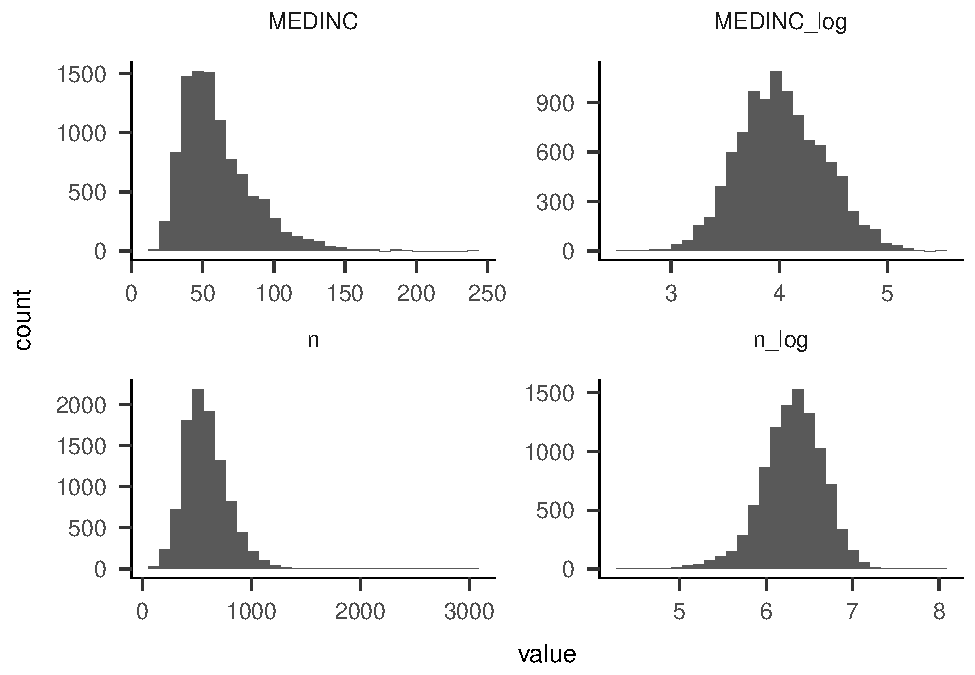
\includegraphics{Method_files/figure-latex/dists-1.pdf}
\caption{\label{fig:dists}Comparison of covariate distributions and their
log transformations.}
\end{figure}

\begin{figure}
\centering
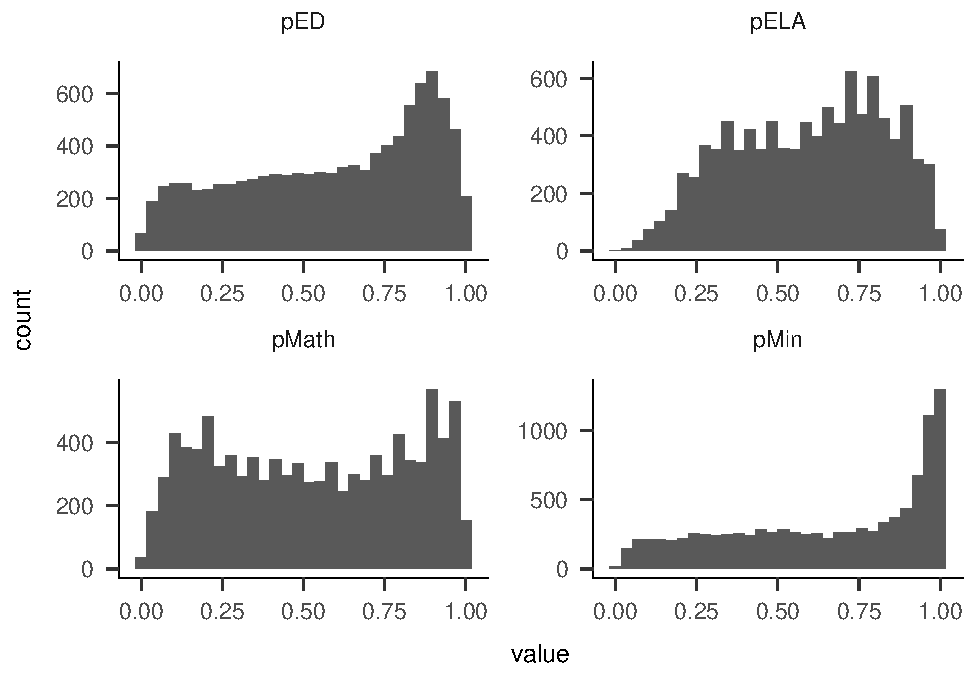
\includegraphics{Method_files/figure-latex/dists2-1.pdf}
\caption{\label{fig:dists2}Distributions of the remaining covariates.}
\end{figure}

\subsubsection{Variable Transformations}\label{variable-transformations}

Log-transformation was used on school size (number of students) and
median income. This is done to allow proportional comparisons at the
extremes of the distributions (Hennig and Liao - 2013). For instance,
the difference between two schools with 4000 and 3000 students should be
weighed as much as the difference between two schools with 400 and 300
students when generating clusters. Figure \ref{fig:dists} displays a
comparison of the distribution of these variables and hteir logs. Figure
\ref{fig:dists2} displays the distribution of the remaining variables.
\ref{tab:tbl-desc}

\subsection{SUBS}\label{subs}

Stratification using balanced sampling (SUBS) was performed prior to
simulation because the group of schools in each strata would be static
across conditions except where the balancing model is manipulated. The
set of covariates in both the full model (SUBS-F) and the omitted
variable model (SUBS-OV) include binary indicator variables

\subsubsection{Number of Clusters}\label{number-of-clusters}

Selecting the number of clusters, \(k\), is one of the most difficult
problems in cluster analysis (Steinley, 2006). To date, the most
extensive investigation of methods for determining \(k\) was conducted
by Milligan and Cooper (1985) who analyzed 30 methods. However, aside
from the limited generalizability of this study, many methods are also
innapropriate in the context of non-hierarchical and thus do not support
k-means clustering. Hennig and Liao (2013) argue that the method of
selecting \(k\) should depend on the context of the clustering and frame
the issue as one of obtaining an appropriate subject-matter-dependent
definition of rather than a statistical estimation.

\begin{itemize}
\item
  Everitt (2011), p126
\item
  clusterSim
\item
  Continuous data?

  \begin{itemize}
  \tightlist
  \item
    Calinski and Harabasz (1974)
  \item
    Duda and Hart (1973)
  \end{itemize}
\item
  Steinley, D. (2006a) K-means clustering: a half-century synthesis.
  British Journal of Mathematical \& Statistical Psychology, 59, 1--34.
\item
  Milligan and Cooper (1984)
\item
  list 30
\end{itemize}

\subsubsection{Subs-Full}\label{subs-full}

\newpage

\section{References}\label{references}

\begingroup
\setlength{\parindent}{-0.5in} \setlength{\leftskip}{0.5in}

\hypertarget{refs}{}

\endgroup






\end{document}
